% !TEX root = ../../thesis.tex

% \cleartoleftpage
% \includepdf{../media/chapter_illustration/poppy_prairie_2.pdf}

\chapter{Open diffusion of Poppy} % (fold)
\label{cha:diffusion}

\section{Introduction} % (fold)

Poppy was initially designed with a scientific objective, aiming to be a new experimental platform opening the possibility to systematically study the role of morphology in sensorimotor control, in human-robot interaction and in cognitive development. Yet, until recently it was complicated because building a robot relied on heavy and costly manufacturing techniques. 3D printing has changed the landscape of what is possible: the design of Poppy transposed it to humanoid robotics and we developed complementary open source electronic and software. As we saw in chapter~\ref{cha:changing_morphology}, it allows to explore new body shapes in just a few days.
In addition, it enables and simplifies the experimentation, the reproduction and the modification of the morphology in research laboratories. It also allows collaborative working, sharing and replication of the results between laboratories.

On the scientific aspect, the ambition is to become a reference platform for benchmarking and dissemination of scientific results. Also the simple design of Poppy also targets non-engineering scientists so humanities, biologist and so on can contribute to the robotics field by using Poppy as experimental tool.
Moreover, thanks to the fact that it integrates advanced and yet easily accessible techniques in an embodiment that motivates students and the wider public, this platform also meets a growing societal need: education and training in technologies combining computer science, electronics and mechanics, as well as a training tool to the emergent revolutionary 3D printing process. With its openness, its design and its rather low-cost, Poppy provides a unique context for experimentation and learning of these technologies in a Do-It-Yourself (DIY) approach.
Finally, the possibility to easily modify both the hardware and the software also makes Poppy a useful tool for artistic projects working with interactive computerized installations.

% Poppy is an open source/open science project, even if the technology developed have high potential to be relevant in Art, Education and of course Science, the user community is a paramount of importance. Because the robot and tools own to the community, it is crucial to have a place to exchange idea and works.

The major challenge is now to succeed in the diffusion of the platform in all these fields. As we can see we the Arduino example, the user community is a paramount of importance and both the diffusion strategy and community management tools are critical.

We think this challenge relies on 3 main aspect: create a playful and motivating multidisciplinary community, improve the hardware modularity and integrate Poppy in the maker revolution by using Fablab for production and distribution.


% 1) Parle un peu plus des limites de la plateforme pour le côté science et open science (e.g. il n’y a pas encore d’exemple de résultat fait par un labo et reproduit par un autre avec Poppy; pas encore d’autres papiers d’autres labos avec Poppy; pas encore de contributions d’autres labos; pourquoi le robot marche pas tout seul et est-ce-que c’est grave?;

% 2) (à mon avis) un élément essentiel du développement de la plateforme dans les milieux éducatifs/FabLabs est le développement de contenus pédagogiques (e.g. le IniRobot de Poppy, peut être fait avec l’ENSAM pour les écoles et Cap Sciences pour les FabLabs) bien mis en avant et accessibles sur le net (e.g. sur le modèle https://learn.sparkfun.com ). Bref, des activités clé en main.

% 3) Evolution du concept “Poppy” dans la tête des gens: Poppy n’est pas “un robot humanoide”, mais une plateforme hard+soft+web+communauté permettant de créer et partager des créatures robotiques diverses (pas forcément humanoïdes, et pourquoi pas des composants comme des moteurs)

% 4) Les moteurs: parler des moteurs open-source



\section{Creating a multidisciplinary community} % (fold)
\label{sec:creating_a_multi}

Toward the creation of such a community, some people are really interesting and have been a great source of inspiration for our work. Among them we can cite Massimo Banzi one of the co-founder of Arduino which spent near 10 years working on the Arduino community. We can also cite Jeff Atwood, co-founder of stack-exchange, he is a software developer who become specialist in creating tools for web community. Along his work he developed a really sight and pragmatic vision of the management of people into a community. The feedback he shares on its blog~\footnote{Jeff Atwood's blog: \url{http://blog.codinghorror.com/}} is really worth reading for anyone wanting to create a community.

The creation of a Poppy's community began when we released Poppy under open source license (October 2013).
The first interaction people has with the project is the website. We managed to create a nice and simple website on \url{www.poppy-project.org} so experts can see potential of the platform while newbies are not afraid by too much technical information.
Yet this website and the open source release draw a lot of attention and we eventually got submerged by emails and the community management. We indeed globally failed to absorb all this enthusiasm, as we were not prepared with adapted community tools such as wiki, forum and so on.

\begin{figure}[tb]
\centering
    \subfloat[][Old BBpress forum]{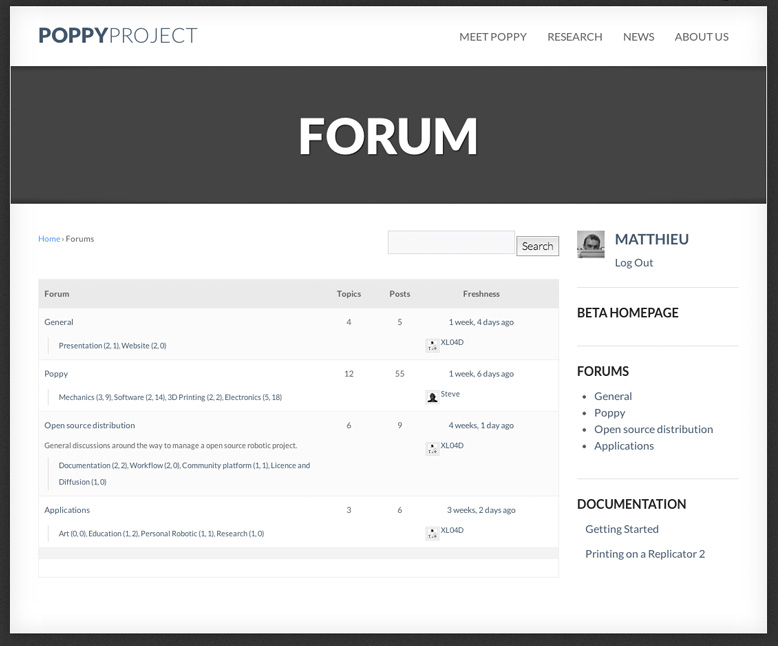
\includegraphics[height=5.2cm]{poppy_forum_bbpress.jpg}}
    \hfil
    \subfloat[][Current Discourse forum]{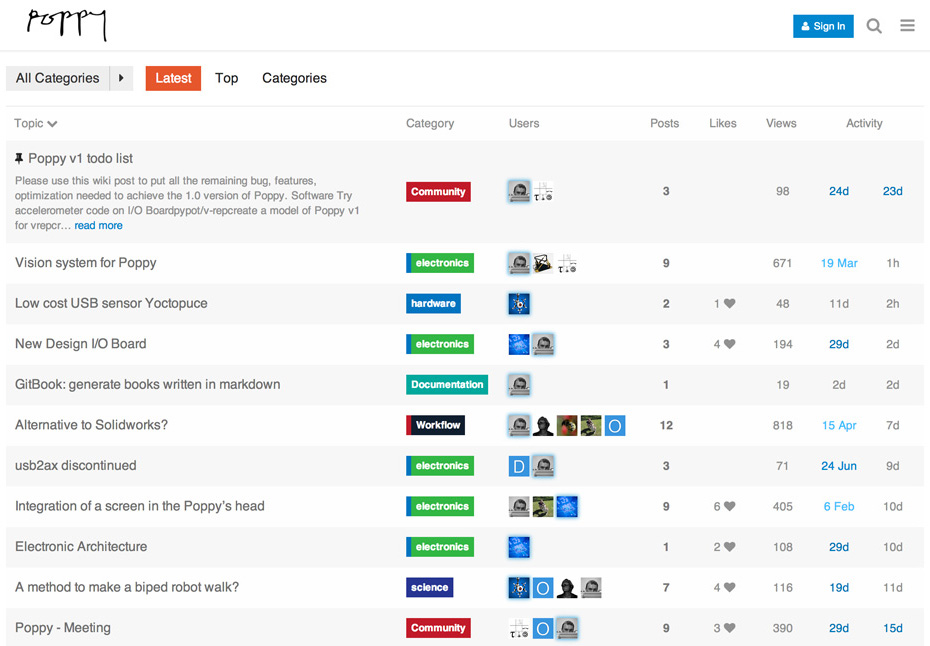
\includegraphics[height=5.2cm]{poppy_forum_discourse.jpg}}
    \caption{Evolution of the forum for the Poppy project}
    \label{fig:poppy_forum}
\end{figure}

Since several months, we set-up a novel forum technology called Discourse\footnote{\url{www.discourse.com}} and created by Jeff Atwood. This forum available on \url{forum.poppy-project.org} greatly help us to manage the community, as it is playful and simple (see \figurename~\ref{fig:poppy_forum}). It is so efficient that we began to use it also for our internal discussions about Poppy's development. These discussions are made public so we can merge time between internal and external communication, extending at the same time the openess of the project.

While this technology solves one of our problems, there are still several others. Firstly, we did not find a wiki technology as simple and playful as Discourse, therefore currently the project clearly lack of documentation (excepted for pypot those documentation\footnote{pypot documentation: \url{poppy-project.github.io/pypot/}} is complete).

Secondly, as science project, we naturally decided to use the English as main language for all communication associated with the project. This implies the main website for presenting the project, as well as support on the forum and the current documentation. However, as we can see in the \figurename~\ref{fig:poppy_community}, english-native people only represent the third of the Poppy's community. While English is usually not a problem for Germanic country, we have been confronted to a lack of contribution from Latin countries on our forum. It is especially the case with French educational and artistic communities those never contributed to the forum even after the successful experiments we have had (see chapter~\ref{cha:education} and chapter~\ref{cha:art}).

Following the Arduino example, we now turned our forum multilingual\footnote(see this topic \url{https://forum.poppy-project.org/t/multi-language-enabled-on-this-forum/304}) by allowing and creating the associated categories for French, German, Italian, Espagnol and Portuguese. We are also currently translating the main website. This work did not yet produce result, but we missed the opportunity during the experiments we had, and we certainly have to wait until new experiments with education and artist to see if we can actually draw more contribution from non-english participants.

\begin{figure}[tb]
\centering
    \subfloat[][]{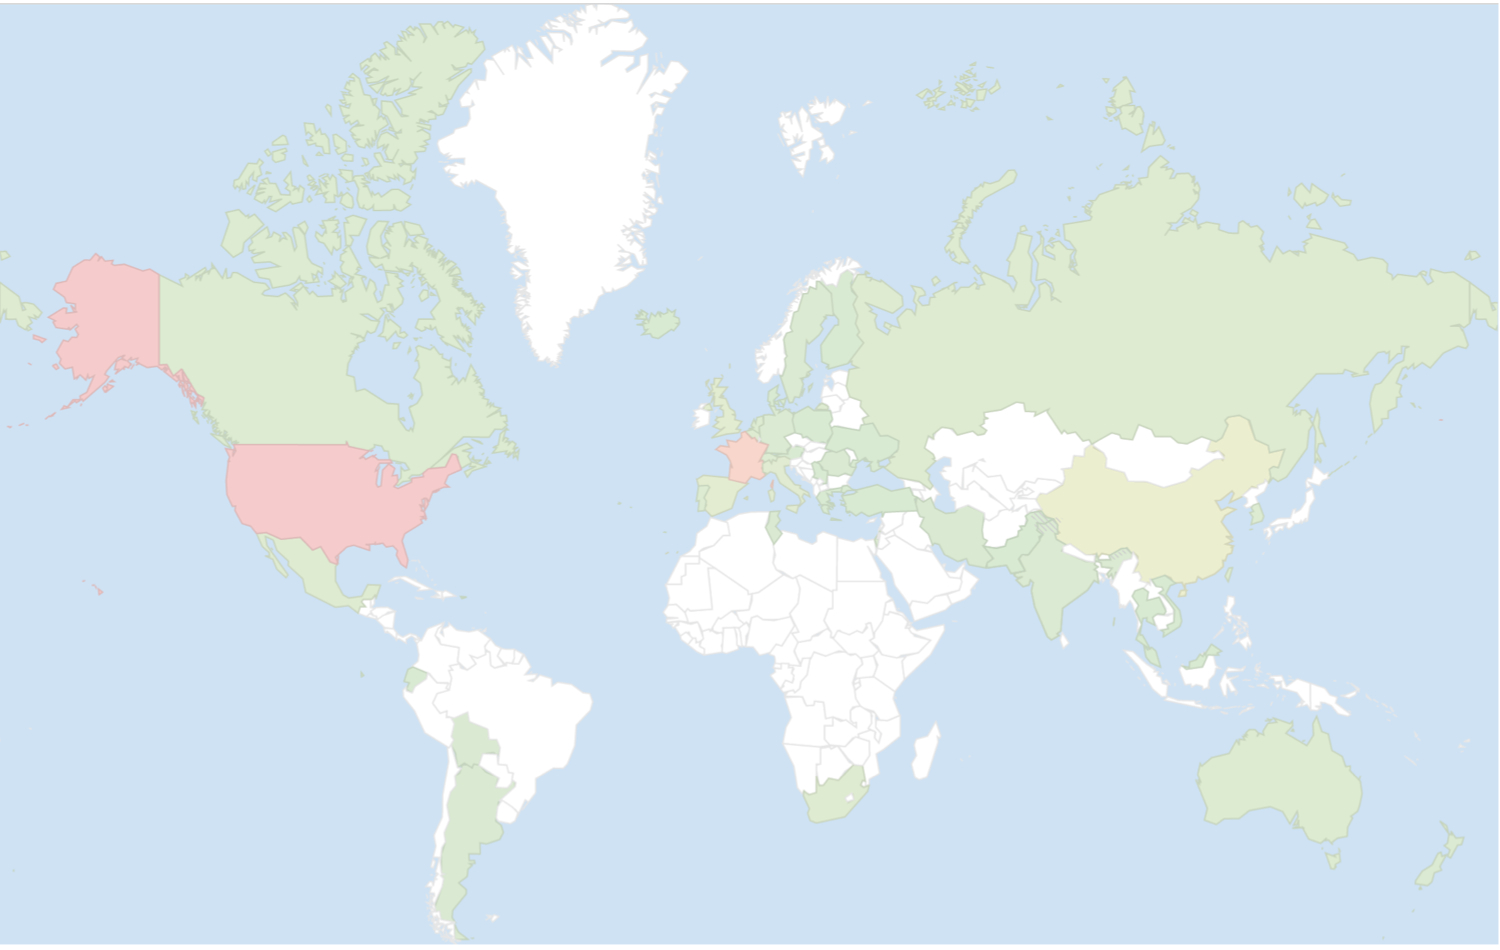
\includegraphics[height=4.5cm]{world_map.jpg}}
    \hfil
    \subfloat[][]{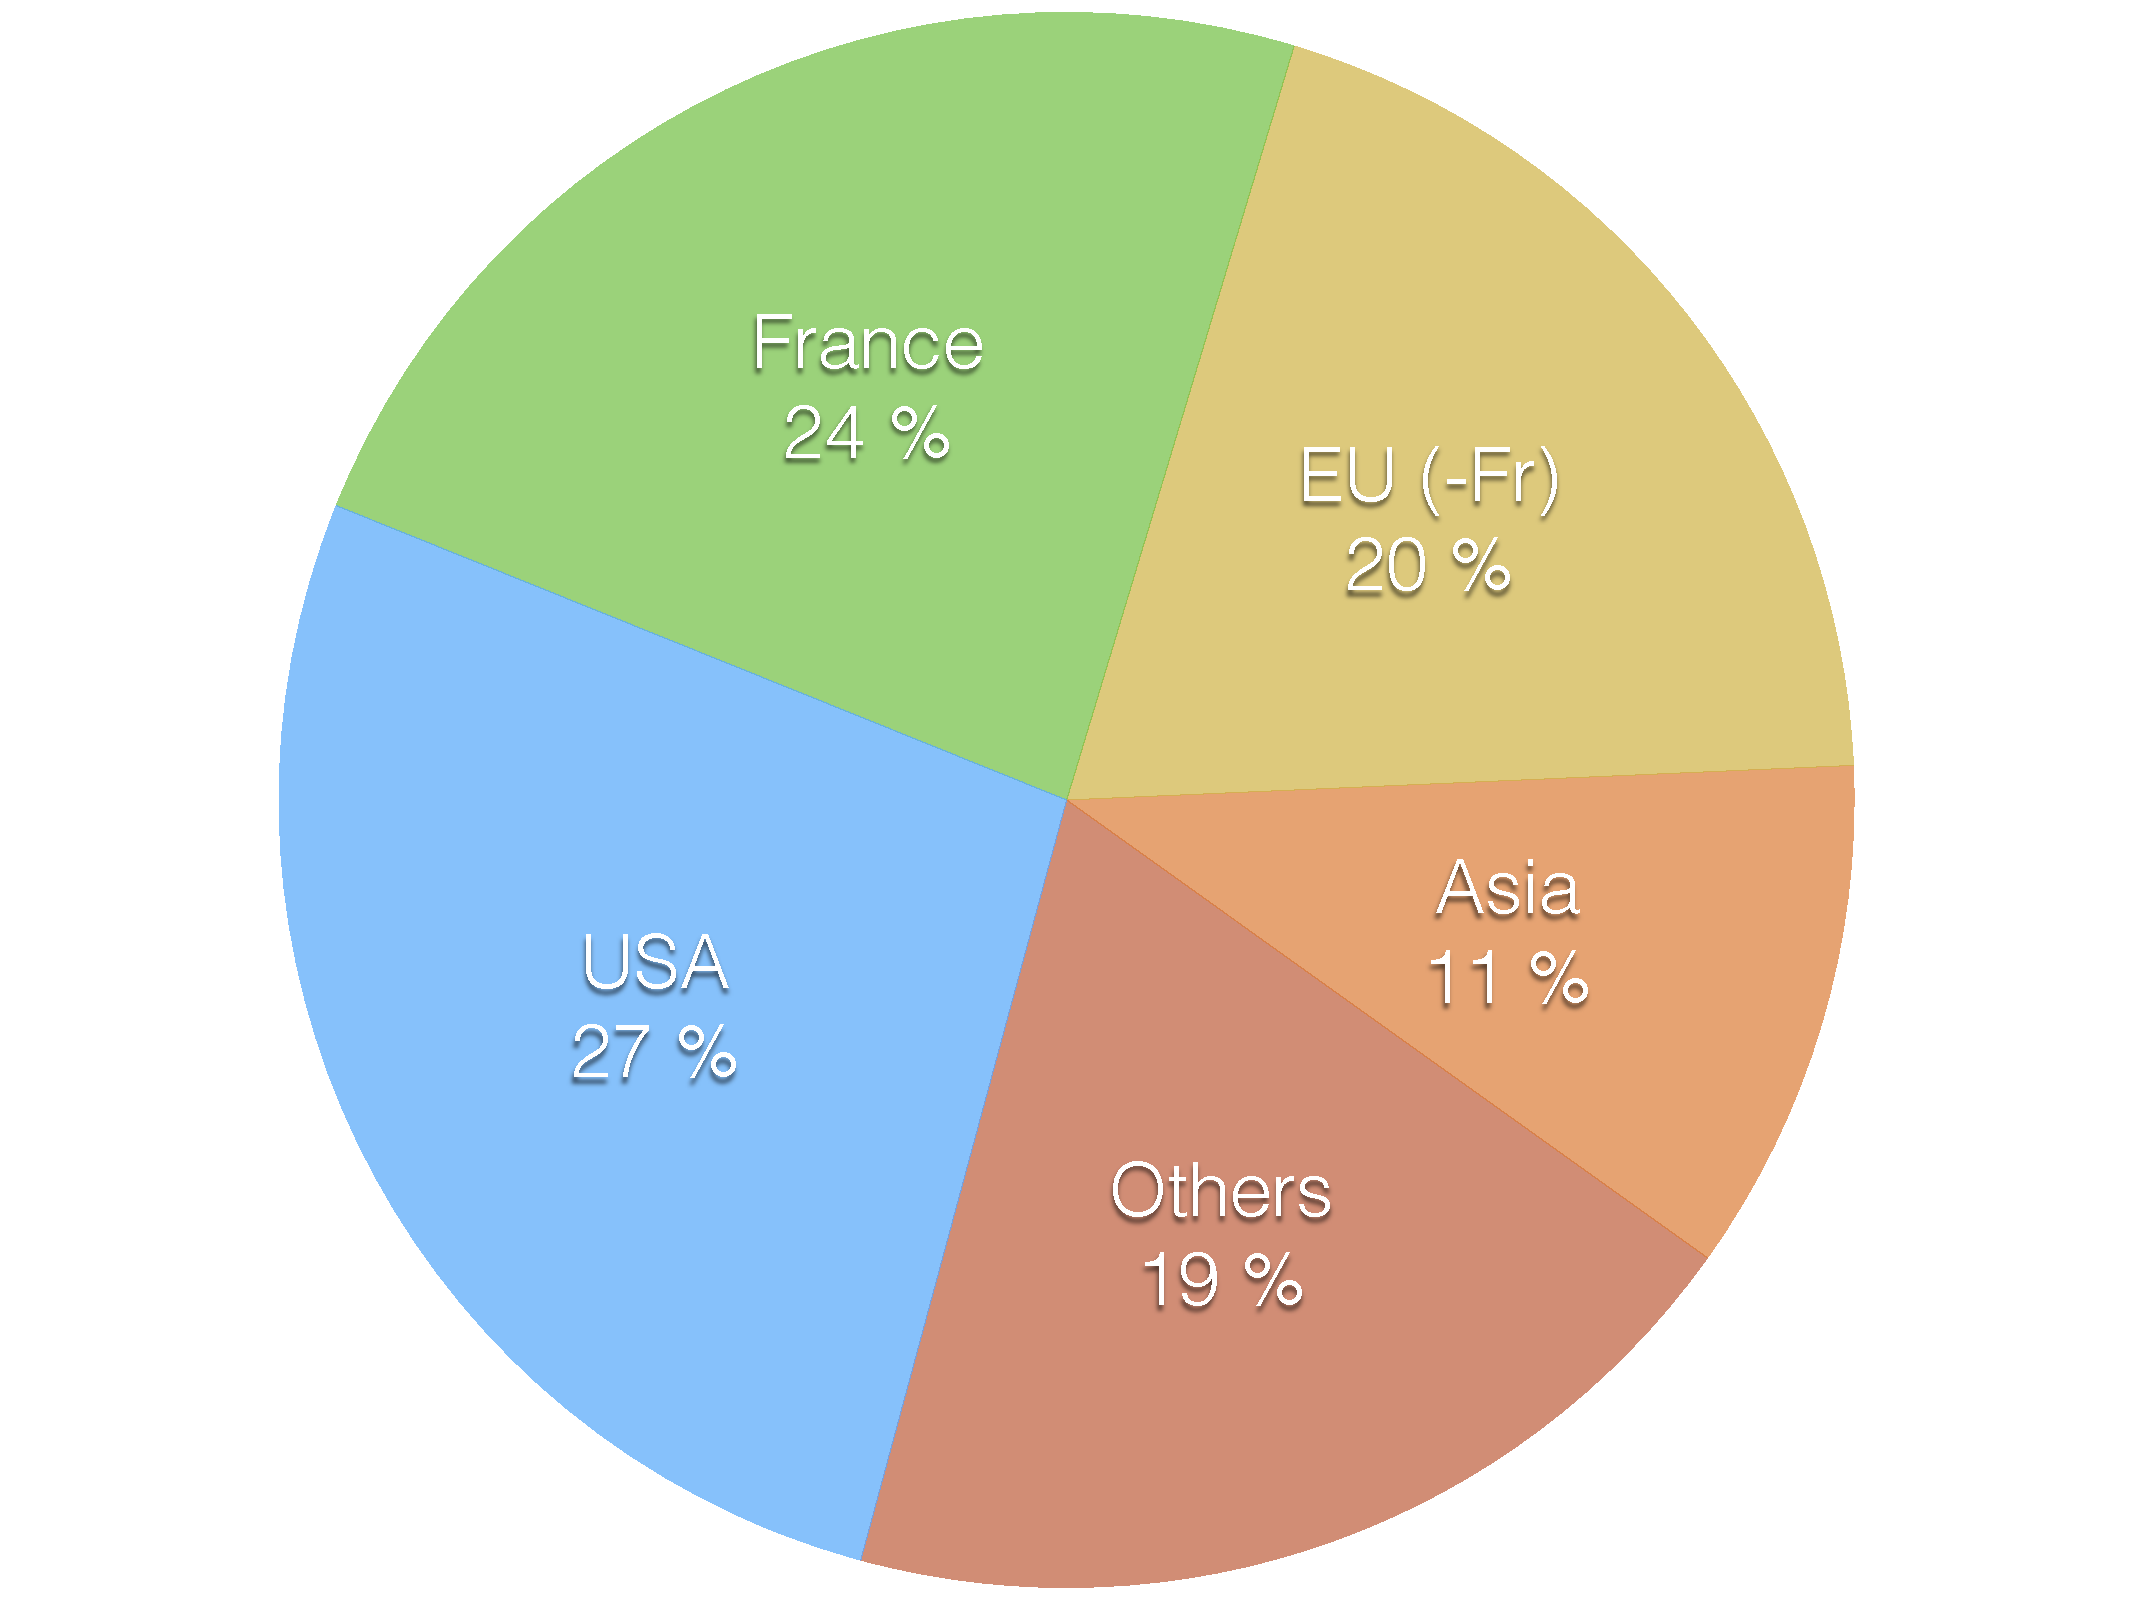
\includegraphics[height=4.5cm]{user_country.pdf}}
    \caption{Activity tracked during October 2013 to February 2014}
    \label{fig:poppy_community}
\end{figure}


Third, creating multidisciplinary community implies that people does not speak the same language and does not have the same technical level. Therefore we will have to improve the accessibility of the project to create a motivational learning curve. This can be achieved thanks to well designed interface, playful content and gamification (\cite{deterding2011game} \cite{groh2012gamification}).


Also we have to take in account the fact people does not read the documentation, described as the paradox of the active user in~\parencite{carroll1987paradox}:
\begin{formal}
    Users never read manuals but start using the software immediately. They are motivated to get started and to get their immediate task done: they don't care about the system as such and don't want to spend time up front on getting established, set up, or going through learning packages.
    The "paradox of the active user" is a paradox because users would save time in the long term by learning more about the system. But that's not how people behave in the real world, so we cannot allow engineers to build products for an idealized rational user when real humans are irrational. We must design for the way users actually behave.
\end{formal}

Jeff Atwood also explained this behaviour with its post on the "just in time theory\footnote{\url{http://blog.codinghorror.com/the-just-in-time-theory/}}" and addressed the problem in Discourse by putting reminder when a user is going to do something maybe wrong, such as summarizing relative topics are forum rules, just when a user is going to post something.

Understanding users needs is very complicated, especially as the Poppy users can be young students, artists or robotics experts. Therefore a major part of the community are not even aware of basic robotic problems such as the motor orientations, the concept of communication buses, the fact motors can burn if too loaded. Thus in addition of a complete documentation (for good student), we will have to work on the just in time reminder so most people can easily assemble and use Poppy.
We already explored some solution for the assembly. For example, motors can be oriented with 16 potential configuration, we need to use one so everyone can share the same robot configuration code (see section~\ref{sec:pypot-robot-abstraction}). We put directly visible indication on the 3D printed parts so user can see how the motor has to be oriented (see \figurename~\ref{fig:motor_orientation}).
\begin{figure}[tb]
    \centering
        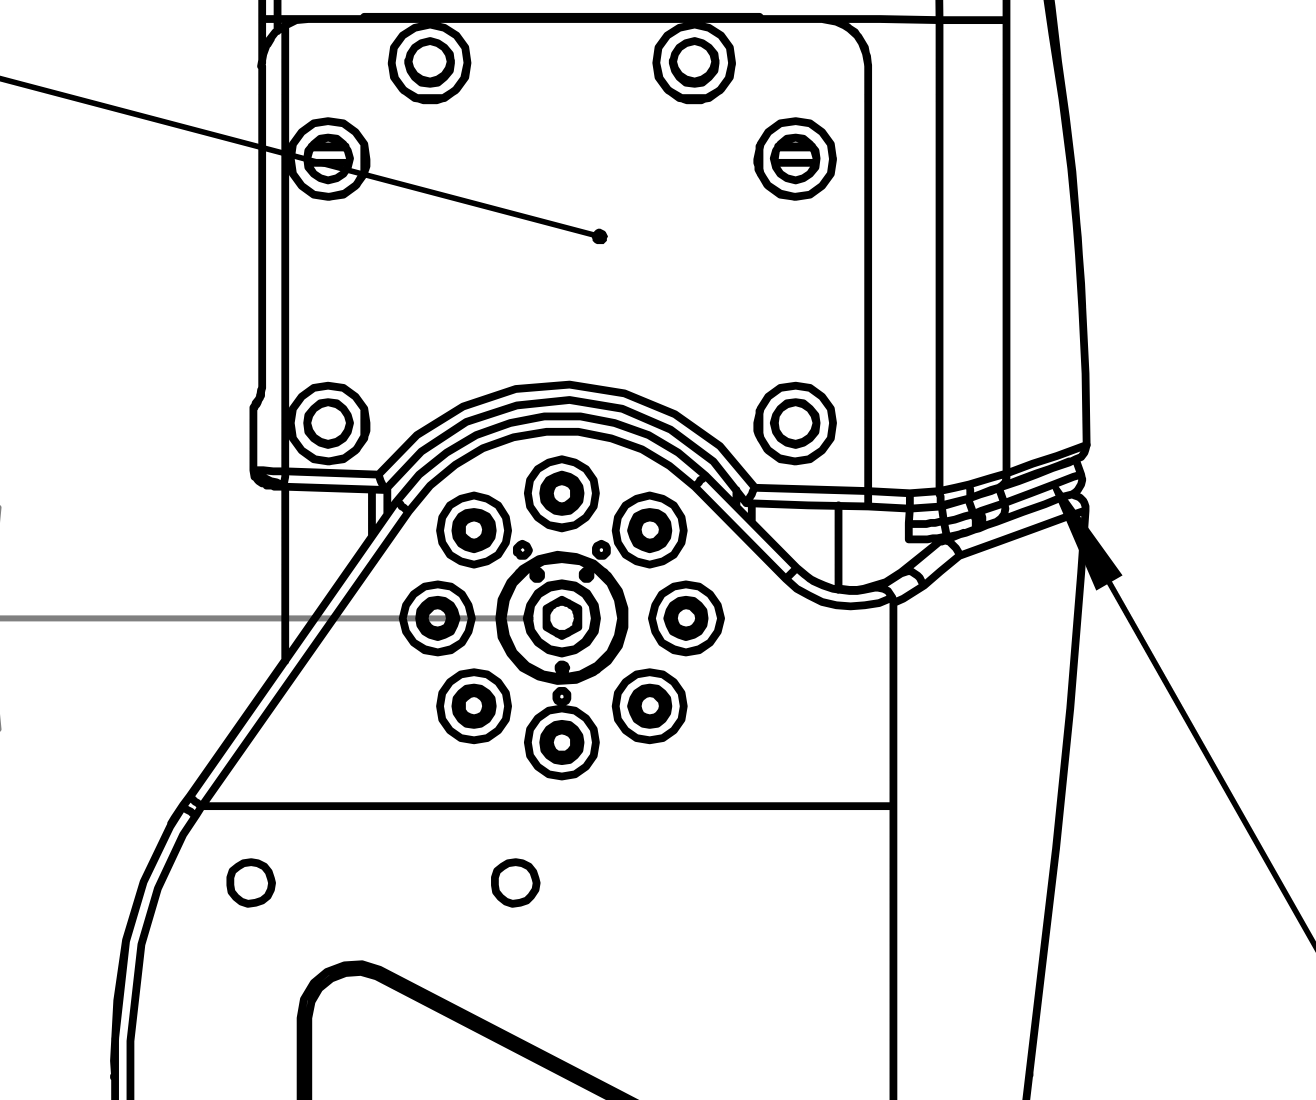
\includegraphics[width=0.6\linewidth]{motor_orientation.png}
    \caption{Image will be update to be more explicit. Yet we can see the 3 points on the motor axis are also present on the part, it is only require to align these point to be sure the motor is correctly assembled. It is kind of "mechanical just in time reminder".}
    \label{fig:motor_orientation}
\end{figure}

Yet this work should be propagated on all elements. On the electronics devices so users has important information (e.g.max voltage, ground/VCC orientation) directly printed on the board, like Arduino did on their boards. On the software so user can be reminded that the primitive paradigms can create undesired behaviours\footnote{The primitive paradigms: The Good, the Bad and the Ugly, see section\ref{sec:pypot-primitives-problems}} as well as being informed when the robot suffers from too much load.


\section{Improving the hardware modularity} % (fold)
\label{sec:improve-hardware-modularity}

As we discussed in details in this thesis, Poppy has a modular morphology. This modularity is expressed with all technologies involved. For the mechanics, we use 3D printing techniques allowing producing quick and low-cost parts. For the electronics, we designed an electronics board based on Arduino allowing to easily plug new sensors. Finally for the software, we built a library using a modular architecture both for the low-level thanks to I/O controllers and for the high-level with primitive paradigm.

As we saw in the chapter REF, this modularity allows for quick experimentation over morphological variants. This functional modularity seems to be enough to allow a wide range of scientific experiments with Poppy and hopefully have real a scientific impact. However, to have an actual impact in the open source community, the technological modularity is essential.

In the software, modularity refers to the manner in which a design is decomposed into different "modules". It is based on the notion of interdependence within modules and independence between modules~\parencite{baldwin2000design}. This concept involves two related ideas: the need to allow work on a given module to be carried out without affecting other modules in the design, a concept known as "loose-coupling", and the need for well-designed "interfaces" between these modules~\parencite{maccormack2006exploring}.

The concept of modularity appears as a fundamental property in the open source software collaboration. Indeed, code modularity allows the overall project to be divided into much smaller and well-defined tasks that individuals can tackle independently from other tasks and without affecting other aspects of the program~\parencite{narduzzo2008modularity}.

Thus Linus Torvalds, emphasized modularity as a design criterion early in the development of Linux~\parencite{dibona1999open}. Indeed without modularity, it would be improbable that contributors could understand the whole design architecture to have a relevant contribution. It would be difficult to add new features or fix bug without affecting other part of the design. Linux needed to be modular to attract and facilitate a developer community. Code modularity allows partitioning of work among a global pool of developers and facilitates the recruitment of new contributors, as it reduces their learning curve to a subset of modules rather than the entire project~\parencite{fitzgerald2004critical}.

Various efforts by corporations selling proprietary software products to develop additional products through an open source approach have been undertaken. One of the most visible of these efforts was Netscape's 1998 decision to make 'Mozilla', a portion of its browser source code, freely available. This effort encountered severe difficulties in its first year, only receiving approximately two dozen postings by outside developers. Much of the problems appeared to stem from the insufficiently modular nature of the software: reflecting its origins as a proprietary commercial product, the different portions of the program were highly interdependent and interwoven.

For twenty years, the open source software development managed to find efficient workflow. There are now tools, rules and guidelines allowing people to develop together new software fluently.

The hardware modularity is not as developed as the software one because it is not possible to abstract the interface. Hardware components have a global shape, connector type and position, and so on, which make difficult to design efficient interface.

\begin{figure}[tb]
\centering
    \subfloat[][Arduino form factor]{\includegraphics[height=3.5cm]{arduino-shield.png}}
    \hfil
     \subfloat[][Google Ara project]{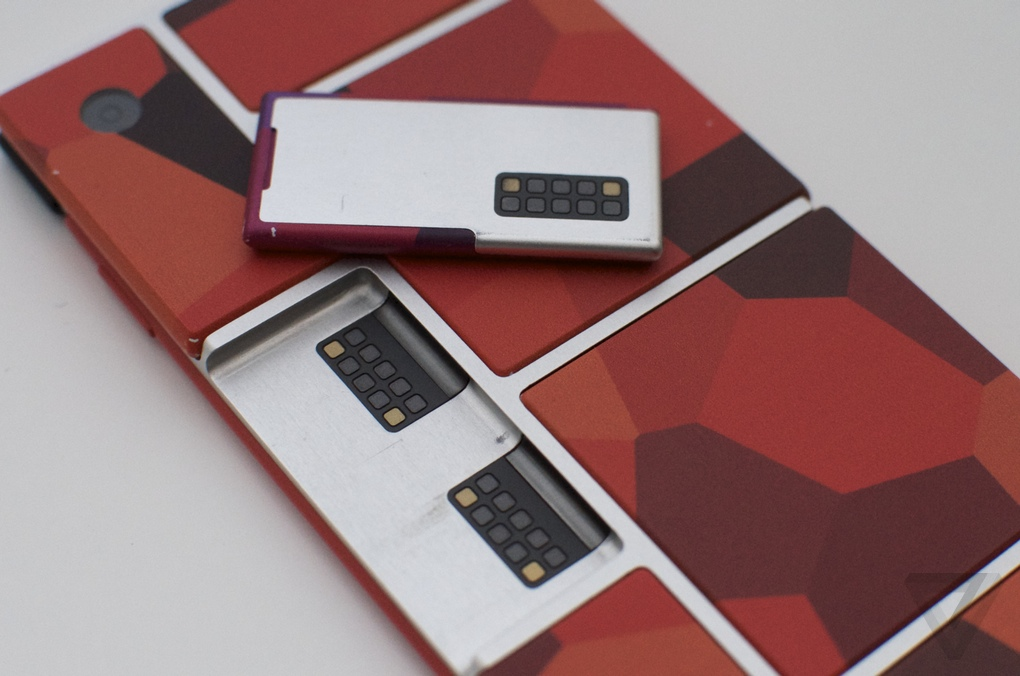
\includegraphics[height=3.5cm]{project-ara.jpg}}\\
    \caption{}
    \label{fig:hardware-modularity}
\end{figure}

Some projects have already addressed these challenges. For example, the Arduino boards (Uno, Leonardo, Yun, Mega, Due) share a same footprint (i.e. where are placed the main I/O pins), in this way any shield developed for one of these Arduino board can also be used on other one. This modularity is a lever arm for the community as potential contributors know that the shield they develop and possibly sell will be compatible we several boards and future ones.
Another example is the Google ARA project, it is a smart-phone with modular elements. It is possible to change only the processor or the camera without having to change the whole phone. To achieve such design, they created interface block (see REF). Therefore any modules following the interface rules can be plugged on the phone.

% Add the fact what people should be able to change easily a part of the robot

To improve the potential impact of Poppy for technology we need to follow such ideas. Indeed the methodology to build Poppy allows for modularity but the actual hardware design is interdependent. The functioning of each mechanical part depends also on element connected to it, for example, the way the pelvis is designed changes the mobility of the legs. Also the particular shape of the IO board and the way connectors are placed, are designed to fit in the current design of Poppy's head.It does not avoid the reuse of such components into other projects but it reduces their relevance.

Thus it would be very useful for a robot platform such as Poppy, made to explore/hack/develop robotics, to easily switch between different technological solutions. On one hand we could test in minute completely different morphologies (new pair of legs for example). On the other hand, and it is maybe the most important point, it would permit to the community to develop their own version of any Poppy's mechatronics systems without having to consider the whole robot structure. By Poppy's systems, we mean legs, feet, arms, hands, torso or head.


Our future technology development will be more oriented toward hardware modularity. This work is already under process for the two main aspect of the robot.

\begin{figure}[tb]
\centering
    \subfloat[][IO Module schematics (under production)]{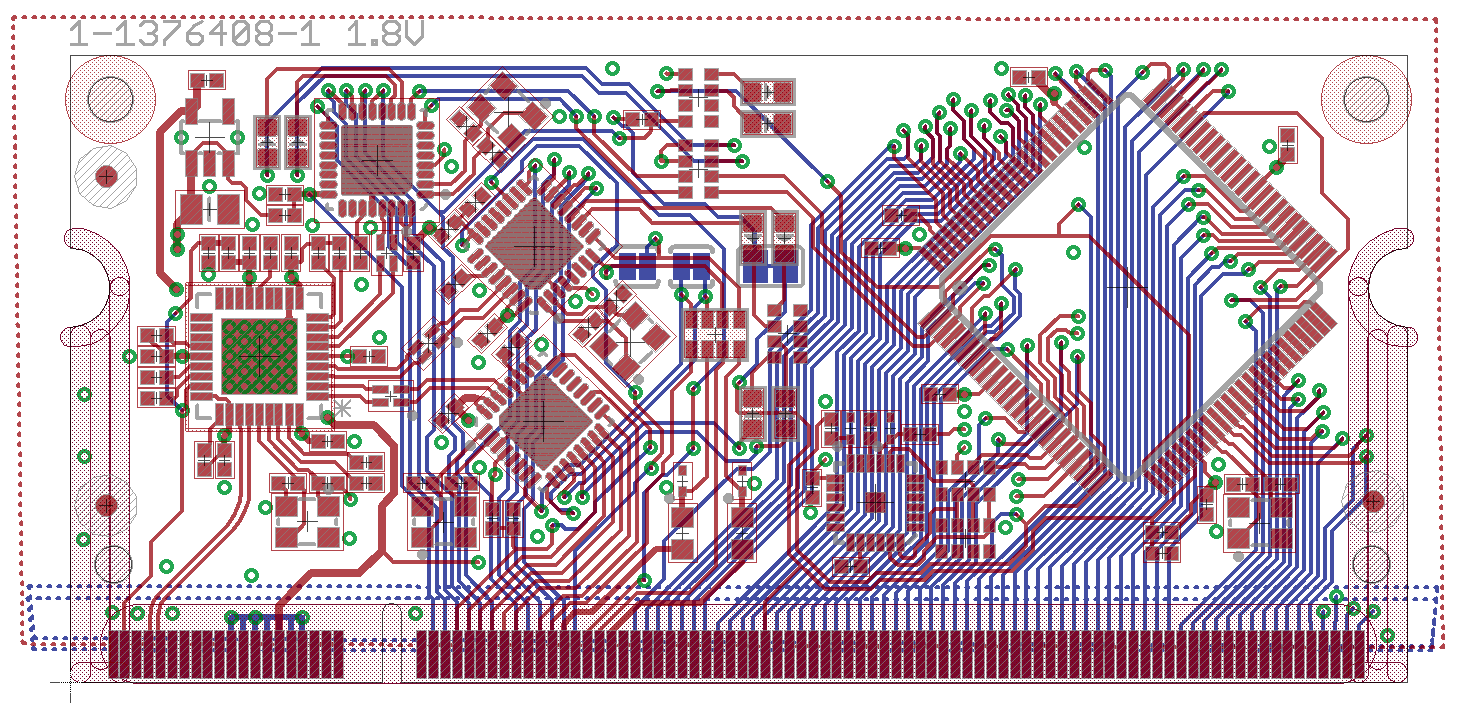
\includegraphics[height=3.5cm]{io-module.png}}
    \hfil
     \subfloat[][Size comparison between the IO board and SO-DIMM format]{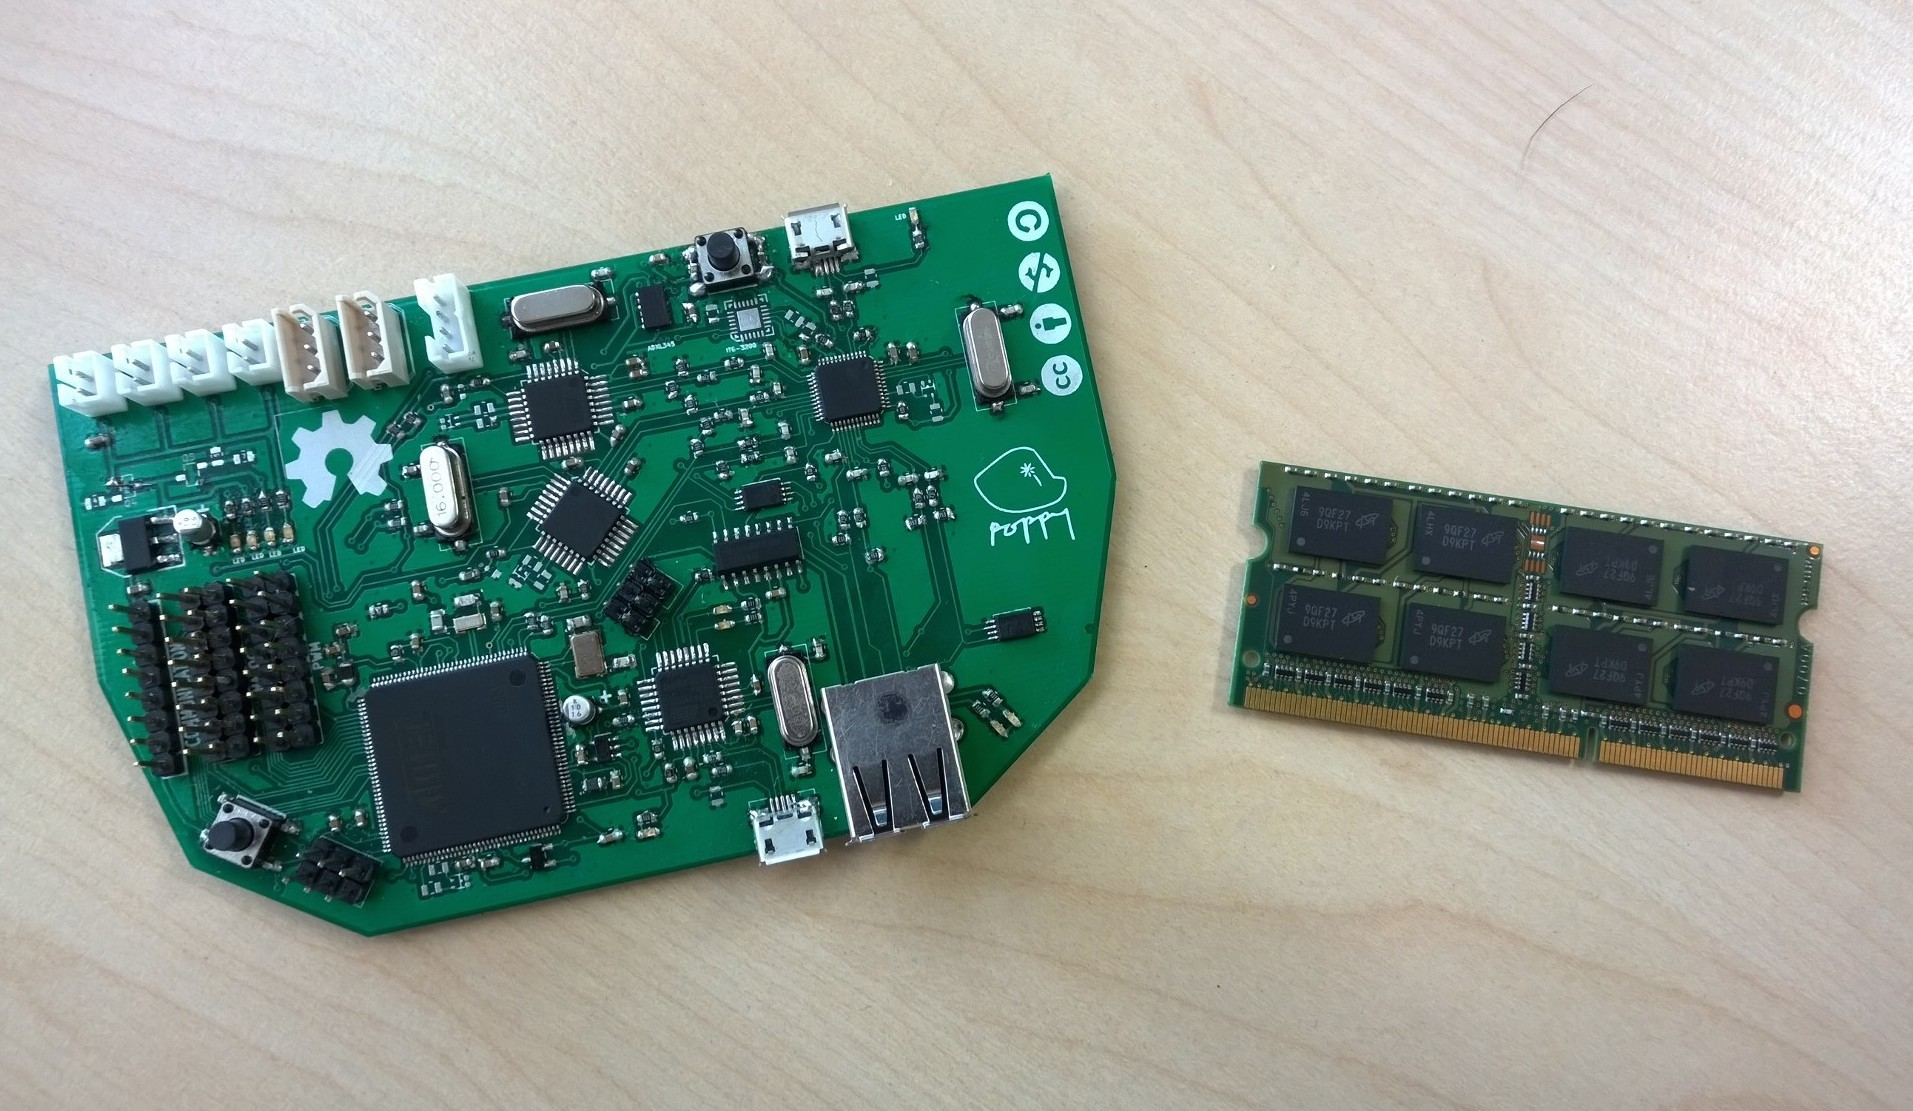
\includegraphics[height=3.5cm]{compare-io-boards.jpg}}\\
    \caption{}
    \label{fig:poppy-electronic-modularity}
\end{figure}

For the electronics, we are also exploring splitting it into modules. We are working on a new design of the IO board, which will involve 2 boards, one IO module with the core of the technology we need (Arduino, motor control) and a shield with connectors.
While the shield is custom to a robot, depending on the needs and motors used, the IO module is very small and versatile so it can be integrate both in small and big robot.
The design of this IO module is already done (see REF) and is based on a DDR2 SO-DIMM format (67x30 mm) with up to 200 pins. This board involves an Arduino Mega with all its GPIO, two modified motor buses compatible for TTL and RS485 communication and an inertial unit MPU6000.


For the mechanics, a first step toward more modularity could be to split the robot into interchangeable sub-modules with defined interface. In this way, contributors could create new design while just having to ensure the interface compatibility. Therefore anyone could create a whole new head or legs system and distribute it so people can test on their Poppy.
We would like to suggest these sub-modules: Head (neck + head), Torso (abs, spine, chest), Arms (both from shoulder to hands) and Legs (both, include pelvis, legs and feet).

Thus it enables a large wide of reconfiguration of Poppy and people are not limited to evolution of current design but can create completely new morphology while being compatible with other Poppy's modules.
For example we could have several locomotive system such as two legs, one jumping leg, wheels, 4 legs (centaur) or just a static base.

While the overview of the module seems clear for us, the details are still a bit muddled. Typical examples are the arms, the functional distinction is not clear. In the current version of Poppy, one of the arms motors is in the torso. On a functional point of view, it should be integrated in the "arms" sub-modules, but on a practical aspect it implies you cut a huge part of the torso and will greatly complicate the interface design.

Another point is the pelvis/torso interface, on one hand, it would be simpler to consider the abs motor as the interface, on the other hand, we do not want to enforce having an abs motor for other submodules.

These kinds of submodules still raise a limitation because the interface has a fixed size, which will constraint the overall size of the robot elements. It should be possible to create a bigger robot, maybe until 120cm but it will be difficult to have a smaller robot than 60cm while keeping the same interface.



\section{Production/Distribution: an alternative approach} % (fold)

Poppy includes three main parts: its mechatronic structure (skeleton and motors); its electronics; its software.

Reproducing and rebuilding the mechatronic structure is easy: the open-source skeleton can be printed on personal 3D printers (or using online services for higher quality printing), and motors are bought off-the-shelf (motors are currently not open-source, but very standard). Obtaining and using the software is very easy: just download on the Poppy web site.

But the fabrication of electronics is a bit more challenging. It is not yet possible to produce electronics components at home, and many institutional users do not have the competence or motivation to do so. There are some kick-starter projects going on a way to facilitate the process, yet they are not ready and won't be ready until a couple of years. The current classical approach to build and distribute this electronics boards is to rise funding allowing the manufacturing of hundreds of boards, which can then be sold by a distribution company. New online platforms such as CircuitHub allow to easily producing one to thousands of board. Yet the cost is exponentially decreasing and unlike the 3D printing. But a French research institute like Inria is not a distributor, it cannot raise funding to "mass" produce electronic components before reselling them. Is not even legally allowed to do it.

Indeed, the mission of a research team at Inria is to do research, and find ways to apply and transfer the results of this research, but not directly to produce and sell a commercial product. If a commercial product can emerge from our research, one way to exploit it is to create a start-up company which will set up a business plan around it, probably based on a production in Asia and then a worldwide distribution to research laboratories, universities and fablabs (see Figure \ref{fig:classic})

\begin{figure}[ht]
    \begin{center}
        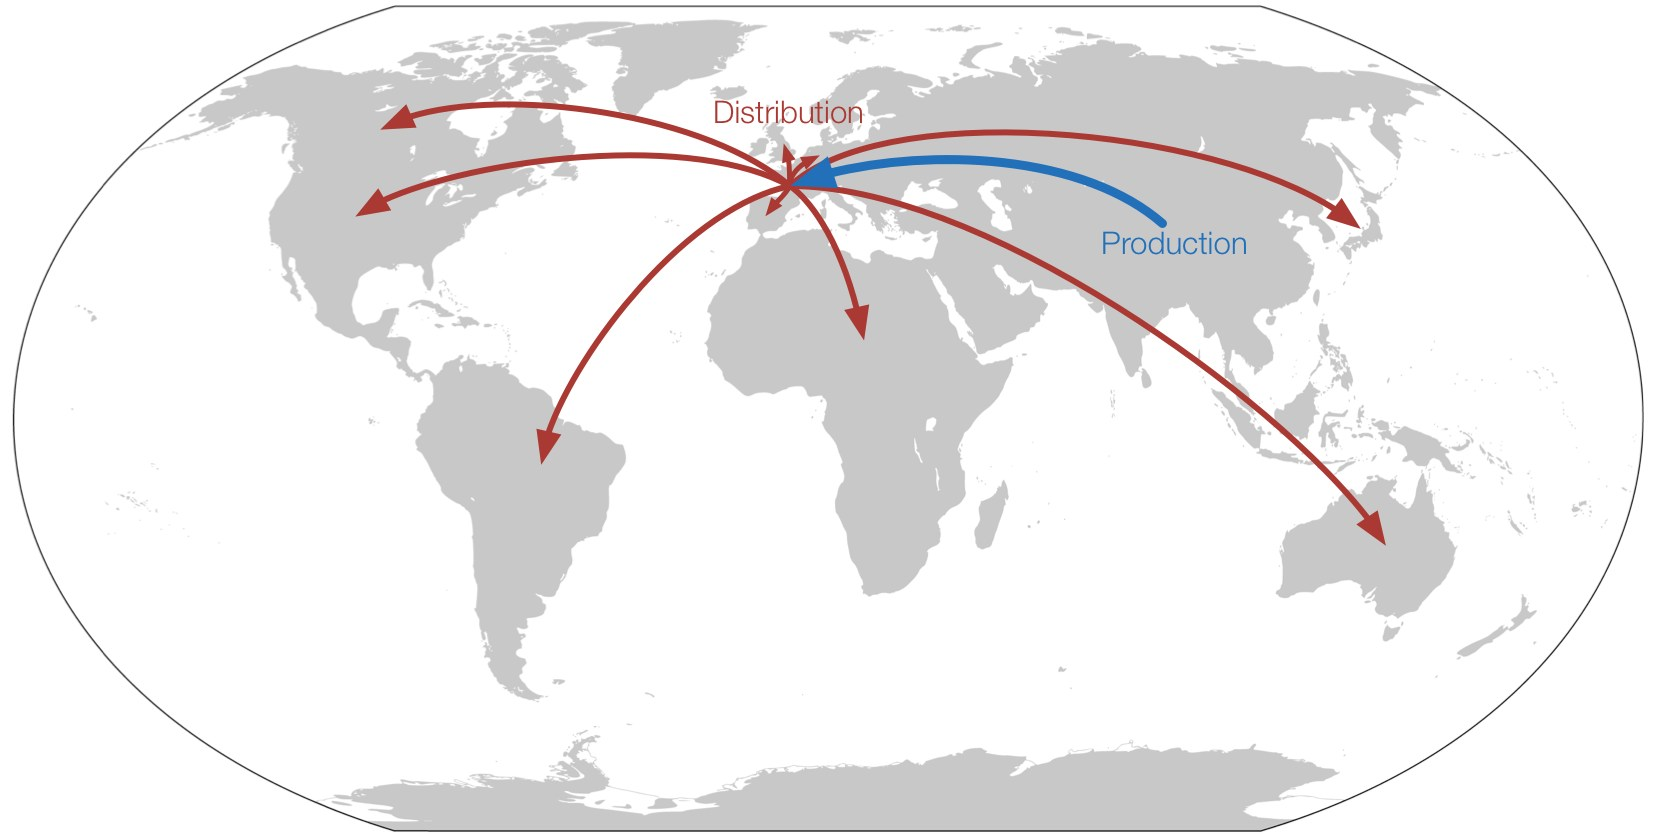
\includegraphics[width=14cm]{classic_production_distribution.jpg}
    \end{center}
    \caption{Classical approach for technology production and distribution}
    \label{fig:classic}
\end{figure}

But Poppy is not designed to be a standard commercial product. While it might foster the creation of an economical ecosystem and jobs, its main purpose is to become an educational tool that remains open, as well as rather low cost and easily reproducible. If the goal had been to make it profitable, it would be necessary to sell it at a much higher price. The robot wouldn't be as accessible at it should to ensure the achievement of its scientific diffusion and educational missions... We would loose the intrinsic purpose of Poppy.

That being said, some users (e.g. artists) might want to obtain and use an already fully assembled Poppy robot and the selling of already prepared kits can be a lever arm for the diffusion of the platform in the research community.
Also, one of the main purposes of Poppy is to be hacked and modified, while some people have all the tooling needed, other can find useful, even if it is charged, to have external support.

On one hand, the use of classic distributors actors is of course the most direct solution and such process are already on the way to permit a commercialization of Poppy's kits for the end of this year. On the other hands, there are novel emerging actors whose could add more sense to the distribution of Poppy.


\subsection{Toward local open factories} % (fold)

Meanwhile, the "makers revolution" is gaining momentum~\parencite{anderson2012makers} and more and more Fablabs are created around the world. As one of the main missions of Poppy is to be a novel educational platform, Poppy could become a popular platform used, hacked, and transformed within the natural FabLab activities. But also, and this is the direction explored below,  it would make sense that Poppy, as a whole or subsets of its components, be produced and distributed by Fablabs, and thus becoming a tool used by Fab Lab to develop and robustify the economic ecosystem in which they live.

An original and constructive organizational process would be to take advantage of the production phase for educational purposes. In this context, each fablab would have the possibility to produce, assemble and sell Poppy to local actors (see Figure \ref{fig:world_fab}). while the production phase could become a training support for the use of 3D printing techniques and the manufacturing of electronic circuits, and later on be exploited through selling the constructed platforms.

\begin{figure}[tb]
    \begin{center}
        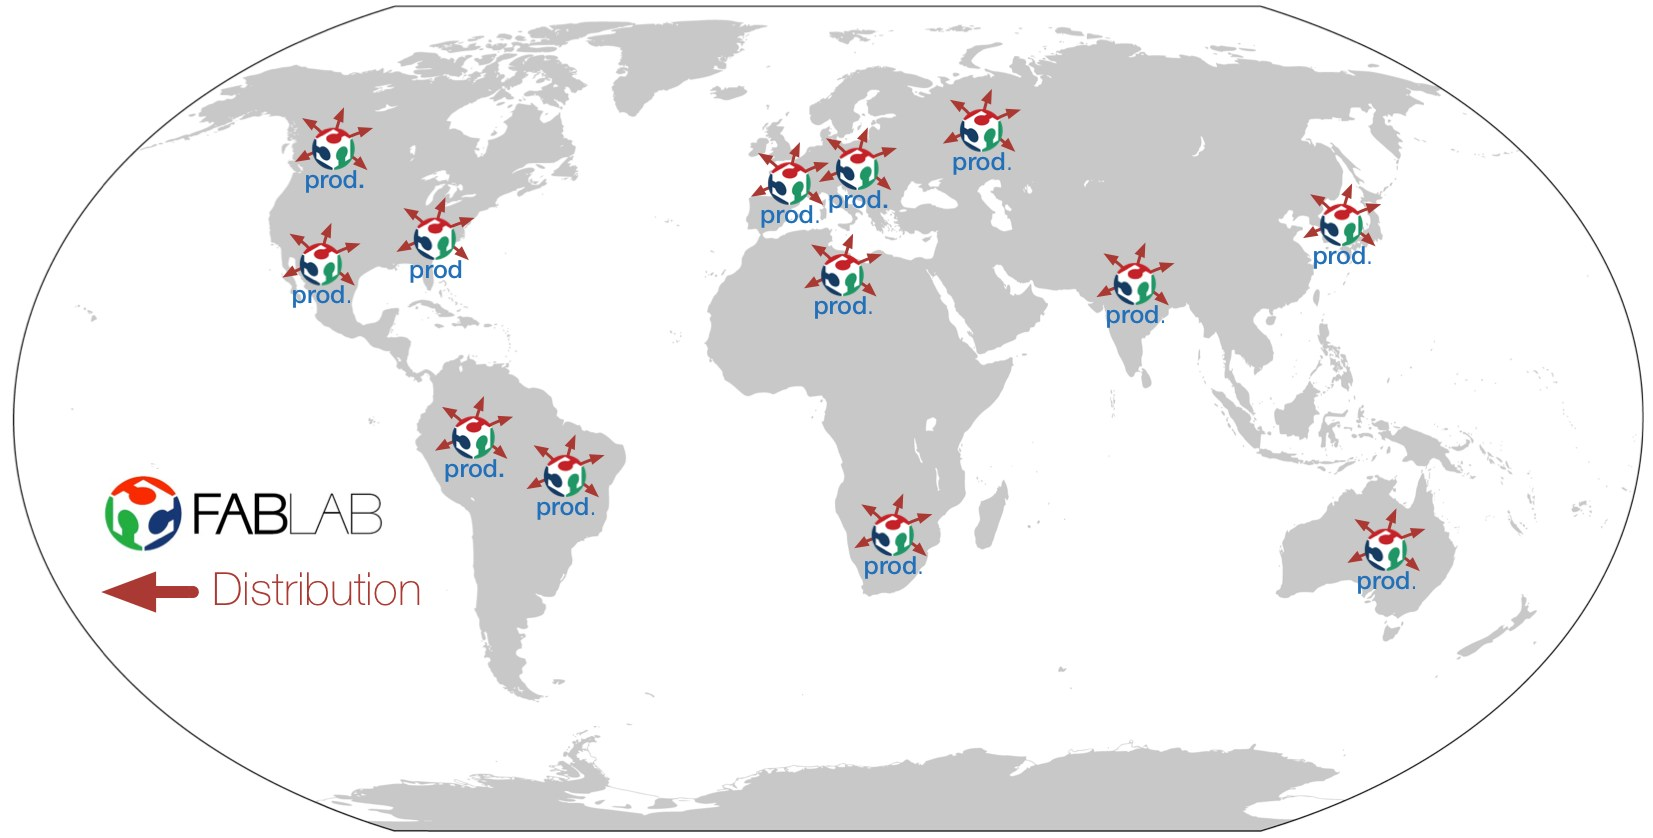
\includegraphics[width=14cm]{fabusine_distribution_world.jpg}
    \end{center}
    \caption{Fabrication and distribution locally done by Fablabs}
    \label{fig:world_fab}
\end{figure}


Also in a context where fablabs need to find an economic model, several sources of income may be found thanks to the distribution of platforms such as Poppy. The first and most obvious one is the sale to local actors of fully-assembled and functional Poppy robots produced by the Fablab. But a more advanced model can emerge. Poppy is a development robotic platform: it means that it can and will be broken, meaning that Fablabs may extend theirs commercial offers. Among them we can cite:

\begin{itemize}
    \item Ensure a support (repairs, upgrades, ...) and may sell maintenance contracts with labs/school/university and even other 3rd party FabLabs.
    \item Provide a customization service to adapt Poppy to specific needs (e.g. a university or lycée that would like to have a Poppy on wheels rather than legs)
    \item For an event or artist residency: The FabLab could rent a robot and provide a technician,
    \item Propose professional formation to 3D printing to companies
\end{itemize}

From these kinds of interaction, links and collaboration between local actors and Fablabs may emerge leading to other potentially funded projects.

\subsection{Promote local collaboration} % (fold)

Beyond the act of production and sales, Poppy could become a pretext to promote the linkage and exchange between local actors from multiple backgrounds. At the scale of a city or region, we can easily imagine a distribution of roles where several FabLabs could collaborate to build and distribute different parts of Poppy depending on their motivations, skills and equipment.
Also, it helps to connect the fablabs with local actors, public/private research labs, companies, schools/universities or artists (see Figure \ref{fig:local_synergy})

\begin{figure}[tb]
    \begin{center}
        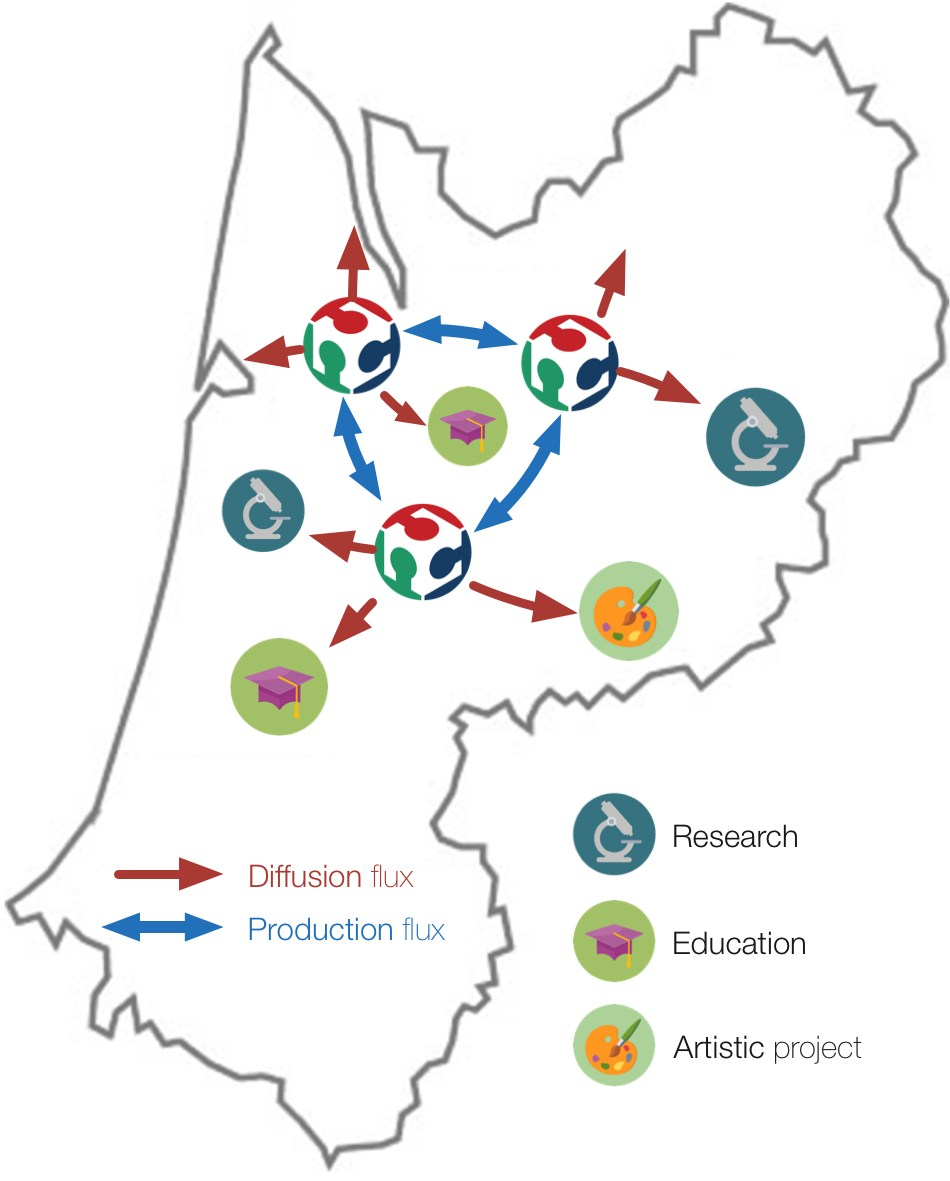
\includegraphics[height=10cm]{fabusine_local.jpg}
    \end{center}
    \caption{A synergy can emerge between Fablabs and local actors}
    \label{fig:local_synergy}
\end{figure}

\subsection{What is the role of the Flowers research team in such a process? } % (fold)

The Flowers research team's role remains essential. As the founders, designers and leaders of both the technological platform and its surrounding philosophy of openness and innovation, the Flowers team continues to improve the platform, take a central role in animating the community of users, and design new uses with scientists, educators, geeks and artists. Within this process, the Flowers team also coordinates the growing of the community of contributors and users, and designs strategies to ensure both the quality and sustainable development of the platform and its uses.

Among the tools used by the Flowers team to ensure such quality and sustainable development is through the control of the "Poppy" brand, and through policies/charters:

\begin{itemize}
\item The "Poppy" brand is owned by Inria, and the use of the brand by 3rd parties like FabLabs will only be possible through agreements ensuring that the Poppy project policies and philosophy is implemented;
\item Agreements take the form of charters/policies between Inria and FabLabs specifying guidelines to follow to ensure both quality and that each party (Inria, FabLab, users) finds its interest.
\end{itemize}

On the Inria side, the creation of an association which role would be to spin-off this technology development, community animation and quality control, is under consideration.



Therefore, Poppy can be one of the first projects launching this new kind of production and distribution process. The last months we met several of the main French FabLab. While there are quite enthusiast with this idea, the organization is not completely ready to go on this way and we will certainly have to use the two ways to distribute Poppy.


% \section{Add educational content} % (fold)
% \label{sec:add_educationnal_content}
% (à mon avis) un élément essentiel du développement de la plateforme dans les milieux éducatifs/FabLabs est le développement de contenus pédagogiques (e.g. le IniRobot de Poppy, peut être fait avec l’ENSAM pour les écoles et Cap Sciences pour les FabLabs) bien mis en avant et accessibles sur le net (e.g. sur le modèle https://learn.sparkfun.com ). Bref, des activités clé en main.

% section add_educationnal_content (end)

% \section{What is Poppy} % (fold)
% \label{sec:what_is_poppy}
% Evolution du concept “Poppy” dans la tête des gens: Poppy n’est pas “un robot humanoide”, mais une plateforme hard+soft+web+communauté permettant de créer et partager des créatures robotiques diverses (pas forcément humanoïdes, et pourquoi pas des composants comme des moteurs)
% % section what_is_poppy (end)


% \section{Open source actuation} % (fold)

% Un potentiel très important a déjà été démontré, mais pour l’exploiter des défis de plusieurs natures restent à relever.

% D’abord, une partie importante de la plateforme est encore propriétaire : les actuateurs actuels sont des moteurs électriques Robotis (Corée) basés sur une technologie mécatronique classique de servo-moteurs contrôlés en position avec des PID. Ces actuateurs ont de fortes limites techniques (pas de contrôle en force, pas de sécurité mécaniquement assurée, ce qui peut être dangereux pour les utilisateurs). Enfin, ils sont chers, leur prix représentant environ 60\% du prix de la plateforme dans son ensemble (chaque moteur coute entre 250 et 300 euros).

% Les limites techniques sont d’abord problématiques pour des raisons scientifiques. En effet, les propriétés mécaniques des moteurs font partie des éléments qu’il doit être possible de contrôler expérimentalement, et il est impossible de le faire avec des moteurs propriétaires. Ensuite, de nombreux aspects essentiels du contrôle moteur ne peuvent être étudiés qu’avec des moteurs contrôlables en force avec une grande bande passante de contrôle. C’est pourquoi par rapport aux objectifs scientifiques du projet, il est essentiel de mettre au point des moteurs basés sur la même approche méthodologique que celle du squelette.

% Avoir des moteurs propriétaires, chers et peu sûrs est par ailleurs un gros handicap pour la diffusion sociétale et éducative de la plateforme. Nous pensons qu’il est possible, en utilisant les techniques de l’impression 3D, de mettre au point des actuateurs (mécanique + contrôle embarqué) plus sûrs, plus performants, et de diminuer le coût d’un ordre de grandeur.

% Aujourd’hui, la plupart des robots réellement performants sont pilotés en force. Une technique très efficace est l’utilisation de pistons hydrauliques. C’est la technologie utilisée par Boston Dynamics sur tous ces robots. Le problème est qu’elle nécessite un réseau hydraulique complex ainsi qu’une pompe puissante afin de mettre l’huile sous pression. Cette solution est très lourde à mettre en œuvre et n’est pas adapté à la réalisation de petits robots ayant vocation à être pratiquement et financièrement accessibles.

% L’approche que nous choisissons est celle de la technologie « Series Electric Actuators ». Cette technologie est basée sur l’ajout d’un ressort à la sortie d’un servo-moteur (voir figure 10). La différence entre la position du moteur et sa sortie est proportionnelle à la force exercée (loi de Hooke). C’est un moyen très simple pour obtenir une mesure directe et précise de la force exercée en sortie. Le contrôle d’un tel système est assez similaire à celui d’un servo-moteur classique.

% Figure 10 - Principe de la technologie "Series Elastic Actuator"
% Bien qu’encore émergente et réservée aux robots construits dans les meilleurs laboratoires du monde, cette technologie devient mature. En effet elle est déjà utilisée dans la plupart des robots de nouvelle génération comme Baxter, Schaft (vainqueur de la première partie du DARPA challenge) mais aussi le robot Meka déjà utilisé dans l’équipe Flowers.

% De plus, le principe de cette technologie étant simple, il existe de nombreuses possibilités techniques de la mettre en œuvre. En effet, actuellement chaque robot utilisant des SEA dispose d’une réalisation technique qui lui est propre. Néanmoins, il apparaît certaines catégories :
%   Une motorisation par câble mis en série avec un ressort de traction qui peut être réalisé de différente manière par exemple : Roboy (figure 11) ou Low-cost compliant manipulator.

% Figure 11 - Mise en oeuvre du principe SEA sur les actuateurs de Roboy
%   Un système à double système ressort-moteur qui permet d’ajuster en permanence la compliance mécanique de l’articulation en modifiant la précontrainte appliquée sur chaque ressort:

% Figure 12 - Exemple d'un actuateur SEA avec double système ressort-moteur pour la réalisation d’une prothèse de jambe
% Un système équivalent à un ressort de torsion en sortie moteur que l’on retrouve par exemple sur COMAN (figure 13) ou sur les robots MEKA. Cette solution permet la réalisation d’actuateurs assez compacts et sera surement le point de départ de la réflexion sur la conception des moteurs de Poppy 2.


% Figure 13 - Actuateurs SEA du robot COMAN

% Malgré ce nombre important de réalisation dans le monde de la recherche, il n’existe à notre connaissance, aucun projet de développement de servomoteurs open source basé sur l’impression 3D et la technologie SEA. Il existe néanmoins un projet open source pour les servomoteurs mais il s’agit uniquement de la partie électronique voir open servo. En ce qui concerne les SEA, on peut trouver des sources d’un gros actuateur (qui utilise des techniques classique de réalisation mécanique) ainsi que des projets fait par des passionnés dans leur atelier. Il existe donc déjà les briques nécessaires pour la réalisation des objectifs de cette ADT. Le challenge sera de les mettre en commun et de produire un design peu coûteux afin de réduire significativement le prix de Poppy 2.




